\documentclass{siproblemset}

% SI Session Information
\course{MTH 1321}       % the course of your SI
\sessionnum{16}         % (optional) specify the session number
\sessiondate{10/27/21}   % the date of the session

\warmup{Concept Review}
\topic{Mean Value Theorem}
\topic{First Derivative Test}
\cooldown{Extrema from Graphs}

% Worksheet Information
\title{Mean Value Theorem\linebreak and Local Extrema}
\sections{Section 4.3}
\withnamespace

\begin{document}
    \maketitle
    
    \activity{Activity 1}{Concavity and Points of Inflection}{Work together in your \textbf{breakout rooms} to answer these questions. Do your best to not refer to your notes while working on these problems.}{30 minutes}
    
    \mcq{For the following functions, (a) find the inflection points and, (b) determine the intervals of concavity.}{
        \task $f(t)=t^3-6t^2+4$
        \Largesp
        \task $y=\theta-2\sin\theta\hspace{0.5cm}[0, 2\pi]$
        
    }
    \newpage
    
    
    \mcq[2]{The following graph is the graph of $f'$, the derivative of the twice-differentiable function $f$. Determine the following:}{
        \task The $x$-values of local extrema
        \task The $x$-values of inflection points
        \task Intervals of increase and decrease of $f$
        \task Intervals where $f$ is concave up and down
    }
    
    \begin{center}
        \mbox{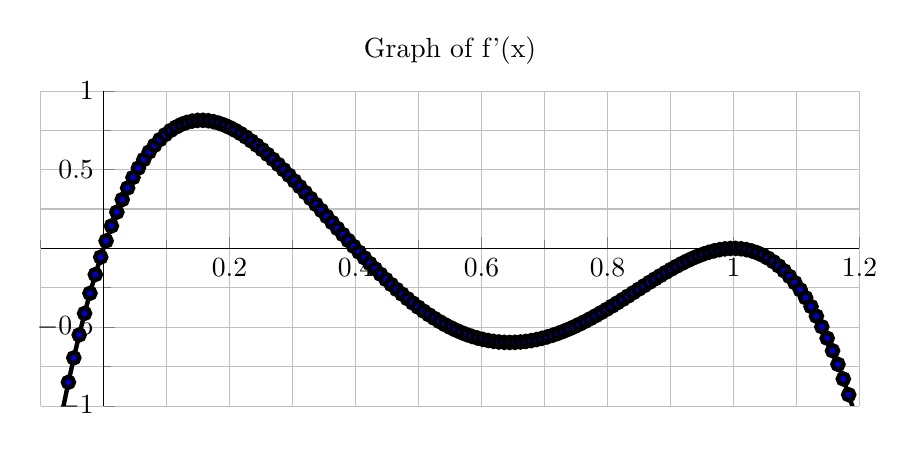
\begin{tikzpicture}[baseline=(current bounding box.north)]
            \begin{axis}[
            title={Graph of f'(x)},
            x=8cm,
            y=2cm,
            xmin=-0.1,
            xmax=1.2,
            ymin=-1,
            ymax=1,
            grid=both,
            major grid style={line width=.2pt,draw=gray!50},
            minor tick num=1,
            axis x line*=middle,
            axis y line*=middle,
            every axis plot/.append style={ultra thick},
            samples=200
            ]
            \addplot+[black, domain=-0.5:1.2] {-30*x*(x-0.4)*(x-1)^2};
            \end{axis}
            \end{tikzpicture}}
    \end{center}
    
    \newpage
    
    \activity{Activity 2}{Second Derivative Test}{Work together in your \textbf{breakout rooms} to answer these questions. Do your best to not refer to your notes while working on these problems.}{30 minutes}
    
    \mcq{For the following functions, (a) find the critical points and, (b) if possible, use the Second Derivative Test to classify them as local minimums, local maximums, or neither. If the Second Derivative Test is inconclusive, state so explicitly and use another method.}{
        \task $f(x)=2x^4-3x^2+2$
        \largesp
        \task $g(x)=(x^2-2)e^{-x}\hspace{0.5cm}$
    }
    \newpage
    
    \activity{Cooldown}{Analyzing a Graph}{Do this problems \textbf{alone}.}{15 minutes}
    \begin{multipartquestion}
        Use the graph below to answer parts (a) through (c).
        
        \begin{center}
            \mbox{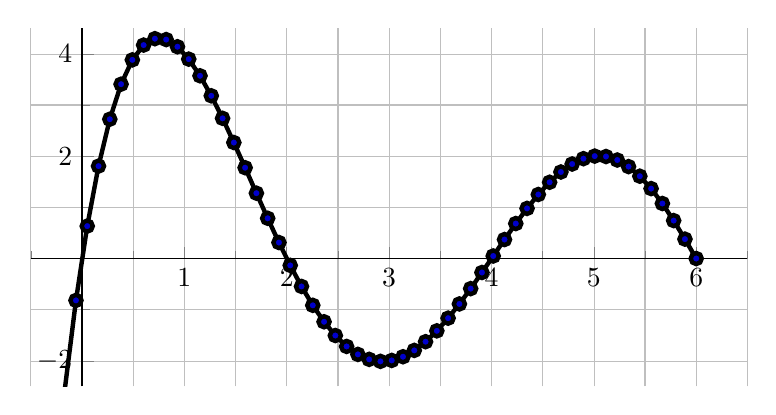
\begin{tikzpicture}[baseline=(current bounding box.north)]
                \begin{axis}[
                x=1.3cm,
                y=0.65cm,
                xmin=-0.5,
                xmax=6.5,
                ymin=-2.5,
                ymax=4.5,
                grid=both,
                major grid style={line width=.2pt,draw=gray!50},
                minor tick num=1,
                axis x line*=middle,
                axis y line*=middle,
                every axis plot/.append style={ultra thick},
                samples=60
                ]
                \addplot+[black, domain=-0.5:6] {13.0667*x-11.9778*x^2+3*x^3-0.0277778*x^4-0.0666667*x^5+0.00555556*x^6};
                \end{axis}
                \end{tikzpicture}}
        \end{center}
        \frq{Assume that the graph above is the graph of $f(x)$. Determine the intervals on which $f'(x)$ is positive and negative. Explain how you got your answer.}
        \Smallsp
        \frq{Assume that the graph above is the graph of $f'(x)$. Determine the intervals on which $f(x)$ is increasing or decreasing and state the $x$-coordinates of inflection points of $f(x)$. Explain how you got your answer.}
        \Smallsp
        \frq{State whether $f(2)$ and $f(4)$ are local minima or local maxima, assuming that the graph above is the graph of $f'(x)$. Explain how you got your answer.}
    \end{multipartquestion}
    
\end{document}